% \documentclass{thesis}
% \usepackage[margin=0.5in]{geometry}
% \documentclass[a4paper,10pt,draft]{thesis}
\usepackage{physics,amsmath, amsfonts, siunitx, amssymb, graphicx, slashed,subcaption}
\usepackage[utf8]{inputenc}
\usepackage[margin=1in]{geometry}
\usepackage[hidelinks]{hyperref}
\usepackage{xr-hyper}
\newcommand{\n}[1]{\nu_{#1}}
\newcommand{\na}{\nu_\alpha}
\newcommand{\nb}{\nu_\beta}
\newcommand{\ana}{\bar{\nu}_\alpha}
\newcommand{\an}[1]{\bar{\nu}_{\text{#1}}}
\newcommand{\anb}{\bar{\nu}_\beta}
\renewcommand{\a}{\alpha}
\renewcommand{\b}{\beta}
\newcommand{\ab}{\alpha\beta}


\renewcommand{\ne}{\nu_e}
\newcommand{\nm}{\nu_\mu}
\newcommand{\nt}{\nu_\tau}
\newcommand{\ns}{\nu_s}

\newcommand{\ane}{\bar{\nu}_e}
\newcommand{\anm}{\bar{\nu}_\mu}
\newcommand{\ant}{\bar{\nu}_\tau}
\newcommand{\ans}{\bar{\nu}_s}

\newcommand{\nee}{\nu_e \to \nu_e}
\newcommand{\nem}{\nu_e \to \nu_\mu}
\newcommand{\net}{\nu_e \to \nu_\tau}
\newcommand{\nes}{\nu_e \to \nu_s}

\newcommand{\nme}{\nu_\mu \to \nu_e}
\newcommand{\nmm}{\nu_\mu \to \nu_\mu}
\newcommand{\nmt}{\nu_\mu \to \nu_\tau}
\newcommand{\nms}{\nu_\mu \to \nu_s}



\newcommand{\Pee}{P_{e  e}}
\newcommand{\Pem}{P_{e  \mu}}
\newcommand{\Pet}{P_{e  \tau}}
\newcommand{\Pes}{P_{e  s}}

\newcommand{\Pme}{P_{\mu  e}}
\newcommand{\Pmm}{P_{\mu\mu}}
\newcommand{\Pmt}{P_{\mu  \tau}}
\newcommand{\Pms}{P_{\mu  s}}


\newcommand{\Pte}{P_{P_{\tau e}}}
\newcommand{\Ptm}{P_{\tau  \mu}}
\newcommand{\Ptt}{P_{\tau  \tau}}
\newcommand{\Pts}{P_{\mu  s}}

\newcommand{\Paeae}{P_{\bar{e}  \bar{e}}}
\newcommand{\Paeam}{P_{\bar{e}  \bar{\mu}}}
\newcommand{\Paeat}{P_{\bar{e}  \bar{\tau}}}
\newcommand{\Paeas}{P_{\bar{e}  \bar{s}}}

\newcommand{\Pamae}{P_{\bar{\mu}  \bar{e}}}
\newcommand{\Pamam}{P_{\bar{\mu}  \bar{\mu}}}
\newcommand{\Pamat}{P_{\bar{\mu}  \bar{\tau}}}
\newcommand{\Pamas}{P_{\bar{\mu}  \bar{s}}}


\newcommand{\Patae}{P_{\bar{\tau}  \bar{e}}}
\newcommand{\Patam}{P_{\bar{\tau}  \bar{\mu}}}
\newcommand{\Patat}{P_{\bar{\tau}  \bar{\tau}}}
\newcommand{\Patas}{P_{\bar{\mu}  \bar{s}}}

\renewcommand{\th}[1][]{%
  \theta\ifx\\#1\\\else_\text{#1}\fi
}
\newcommand{\thm}[1][]{%
  \theta^\text{M}\ifx\\#1\\\else_\text{#1}\fi
}
\renewcommand{\t}[1]{\text{{#1}}}
\newcommand{\avg}[1]{\left\langle {#1} \right \rangle}
\newcommand*{\dm}[1][]{%
  \Delta m^2\ifx\\#1\\\else_\text{#1}\fi
}
\newcommand{\zreco}{\cos{(\theta_z^{reco})}}
\newcommand{\ztrue}{\cos{(\theta_z^{true})}}
\newcommand{\z}{\cos{(\theta_z)}}
\newcommand{\Ereco}{E^{reco}}
\newcommand{\Etrue}{E^{true}}
\newcommand{\Aeff}{A^\text{eff}}
\newcommand{\emm}{\epsilon_{\mu\mu}}
\newcommand{\emt}{\epsilon_{\mu\tau}}
\newcommand{\eet}{\epsilon_{e\tau}}
\newcommand{\eem}{\epsilon_{e\mu}}
\newcommand{\ett}{\epsilon_{\tau\tau}}
\newcommand{\ep}{\epsilon^\prime}


% \begin{document}
\section{The Sterile Hypothesis}
With the null ($3\nu$) hypothesis normalized to the IceCube Monte Carlo as in Eq.~\ref{eq:Nth}, we are now in good shape to study the sterile effect on the probabilities, and how that compares to data.
First, let us see how the collected data from Fig.~\ref{fig:IC_data} deviates from the predicted $3\nu$ oscillations.
\begin{figure}
    \centering
    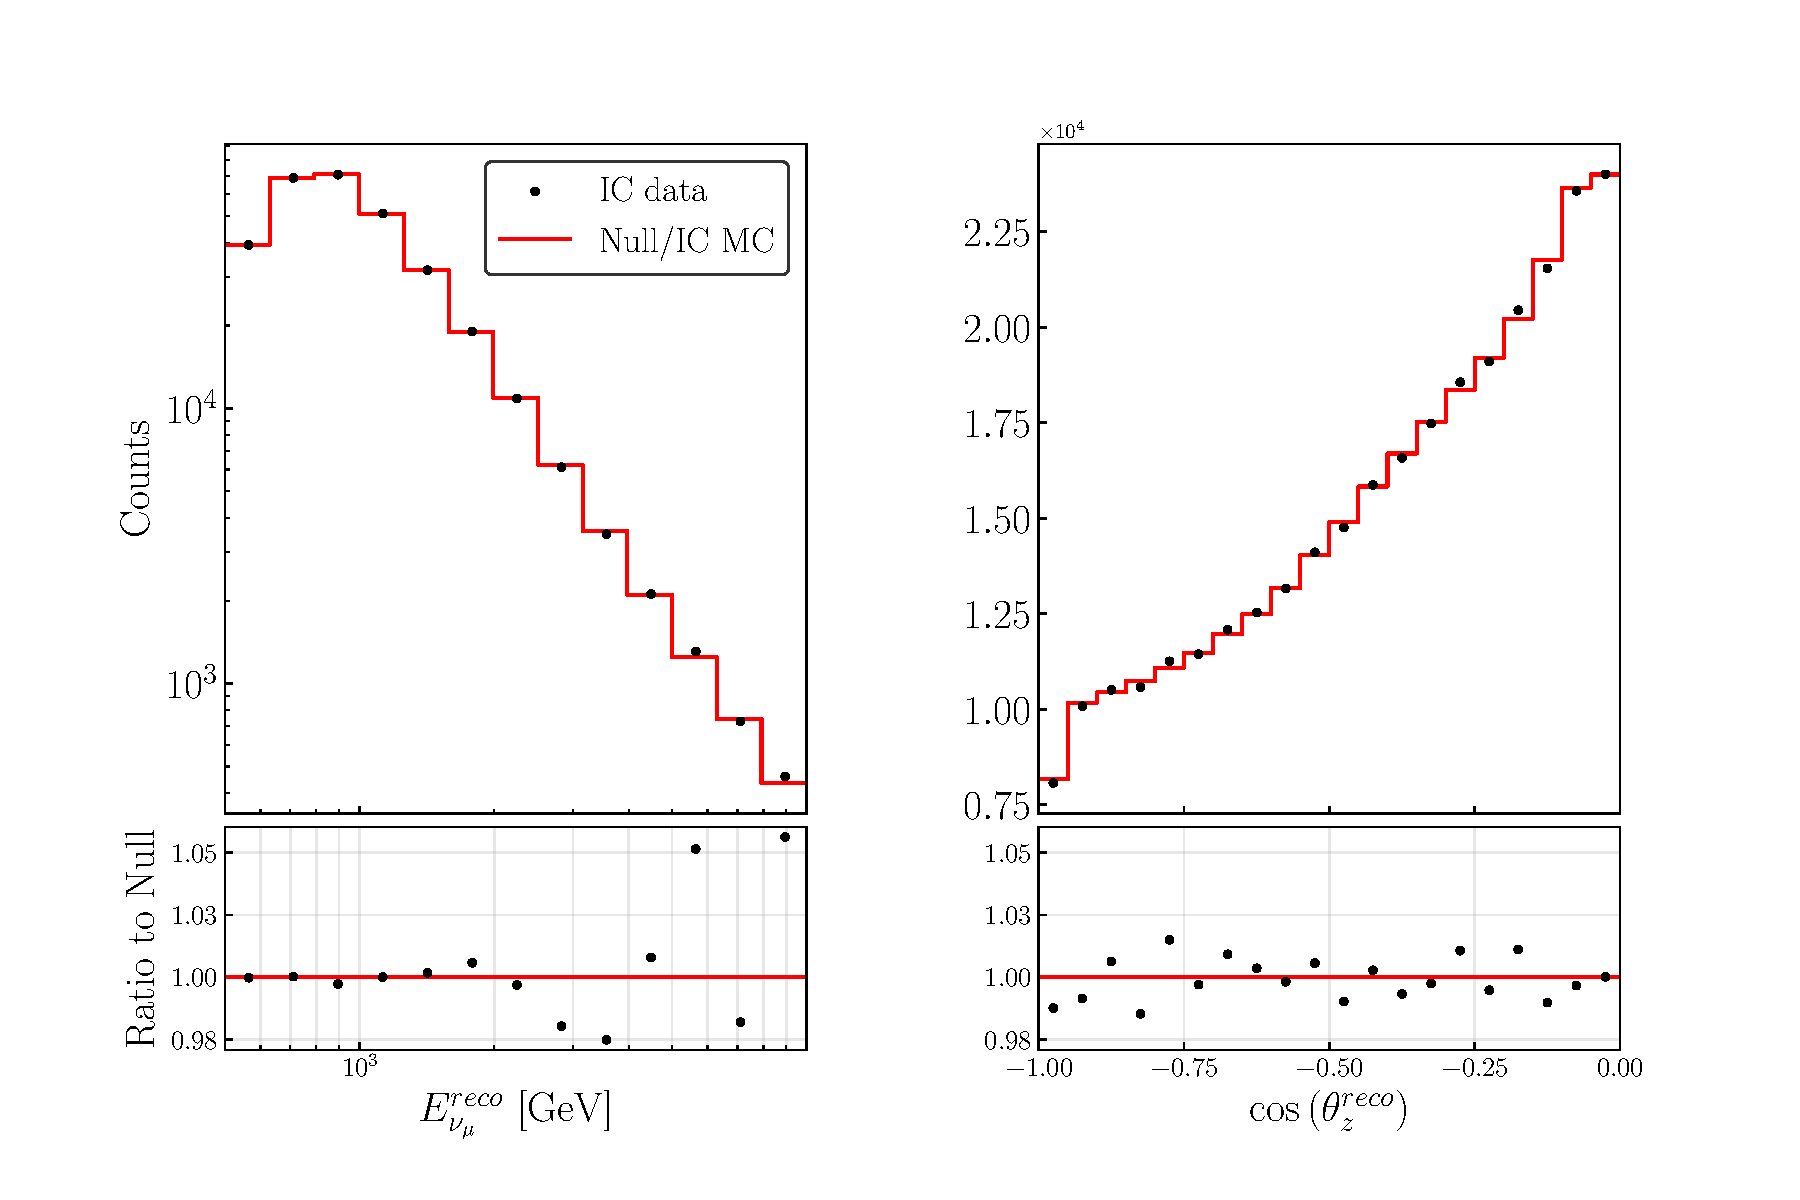
\includegraphics[width=0.8\textwidth]{figures/IC_rates.pdf}
    \caption{}\label{fig:IC_rates}
\end{figure}
Fig.~\ref{fig:IC_rates} shows an impressive agreement to the standard $3\nu$ oscillation picture, with the largest deviations of $~6\%$
for neutrinos close to double-digit \si{\TeV} values. In zenith, the data only deviates $\pm 1\%$. Recalling the \si{\TeV} disappearance from 
Fig.~\ref{fig:sterile_resonance}, we see that we have a similar deficiency found in the data at \SI{4}{\TeV}. Thus, we expect the best fitting 
sterile hypothesis to include a $\dm[41]$ that places the resonant disappearance in the same region. From Fig.~\ref{fig:resonance_shift}, we see
that a mass of $\dm[41] = \SI{1.5}{\eV \squared}$ achieves this. 

\subsection{\texorpdfstring{$\chi^2$}{Chi-squared} Minimization}
For our analyses, we define our $\chi^2$ as
\begin{align} \label{eq:chisq}
    \chi^{2}(\hat{\theta},\alpha,\beta)=\sum_{ij} \frac{\left(N^\text{th}-N^\text{data}\right)_{ij}^{2}}
    {\left(\sigma^\text{data}_{ij}\right)^{2} + \left(\sigma^\text{syst}_{ij}\right)^{2}}+ 
    \frac{(1-\alpha)^2}{\sigma_\alpha^2} + \frac{\beta^2}{\sigma_\beta^2}\,
\end{align}
where we minimize over the model parameters $\hat{\theta}$, the penalty terms $\alpha$ and $\beta$.
$N_{ij}^\text{th}$ is the expected number of events from theory, and $N_{ij}^\text{data}$ is the observed number of events in that bin. 
We set $\sigma_\alpha = 0.25$ as the atmospheric flux normalization error, and $\sigma_\beta = 0.04$ as the zenith angle slope error~\cite{hondapaper}. 
The observed event number has an associated Poissonian uncertainty $\sigma_{ij}^\text{data} = \sqrt{N_{ij}^\text{data}}$.
For IceCube, the event count takes the form
\begin{align}
    N^\text{th}_{ij} = \alpha\left[1+\beta (0.5 + \zreco_i )\right] N_{ij}(\hat{\theta})\,,
\end{align}
with $N_{ij}(\hat{\theta})$ from Eq.~\ref{eq:Nth}. Here, the term $ \beta (0.5 + \zreco_i )$ allows the event distribution to rotate with angle $\beta$ around the median zenith angle of $\zreco = -0.5$.
We also have an uncorrelated systematic error $\sigma_{ijk}^\text{syst}$. We set $\sigma_{ijk}^\text{syst} = f\sqrt{N_{ijk}^\text{data}}$, where $f$ is a percentage of our own choosing,
typically a value between 0 and 20 \%.

The minimization of Eq.~\ref{eq:chisq} simply returns a value for each set of model parameters. We use this value to quantify to what extent
our theoretical simulations $N^\text{th}_{ij}$ agree with the data $N^\text{data}_{ij}$ within the error bounds provided by $\sigma_a,\sigma_b,$ and $f$.
We then select the set of $\chi^2$ values which are the smallest and our allowed parameters are then their associated $\hat{\theta}$.
We then translate the $\chi^2$ distribution by subtracting the best-fit point, and analyze $\Delta \chi^2 = \chi^2 - \chi^2_{min}$.
From the $\chi^2$-distribution, one can show that the $90\%$ confidence level has a value of $2.71$ for two degrees of freedom. When slicing through the 
two-dimensional grid of $\Delta \chi^2$ at this level, we then obtain a contour plot that tells us what regions are within our $90 \%$ and what regions are not.

\subsection{Sterile Mass and Mixing}
Let us start with looking at the best-fit event distribution resulting from the $\chi^2$ minimization.
Fig.~\ref{fig:final_rate_plot} now contains the best-fit event distribution assuming the sterile hypothesis.
The best-fit values are $\dm[41] = \SI{0.01}{\eV\squared}$ and 
$\sin(2\theta_{24})^2 = 0.67$ ($\theta_{24} = \SI{27.5}{\degree}$). %TODO:double check these
The contour plot shown in Fig.~\ref{fig:s24_contour} divides the parameter space into two regions.
To the right of the boundary, the $\Delta \chi^2$ has values above the confidence level, meaning that 
those parameter pairs can be excluded at a certain confidence level.
\begin{figure}
    \centering
    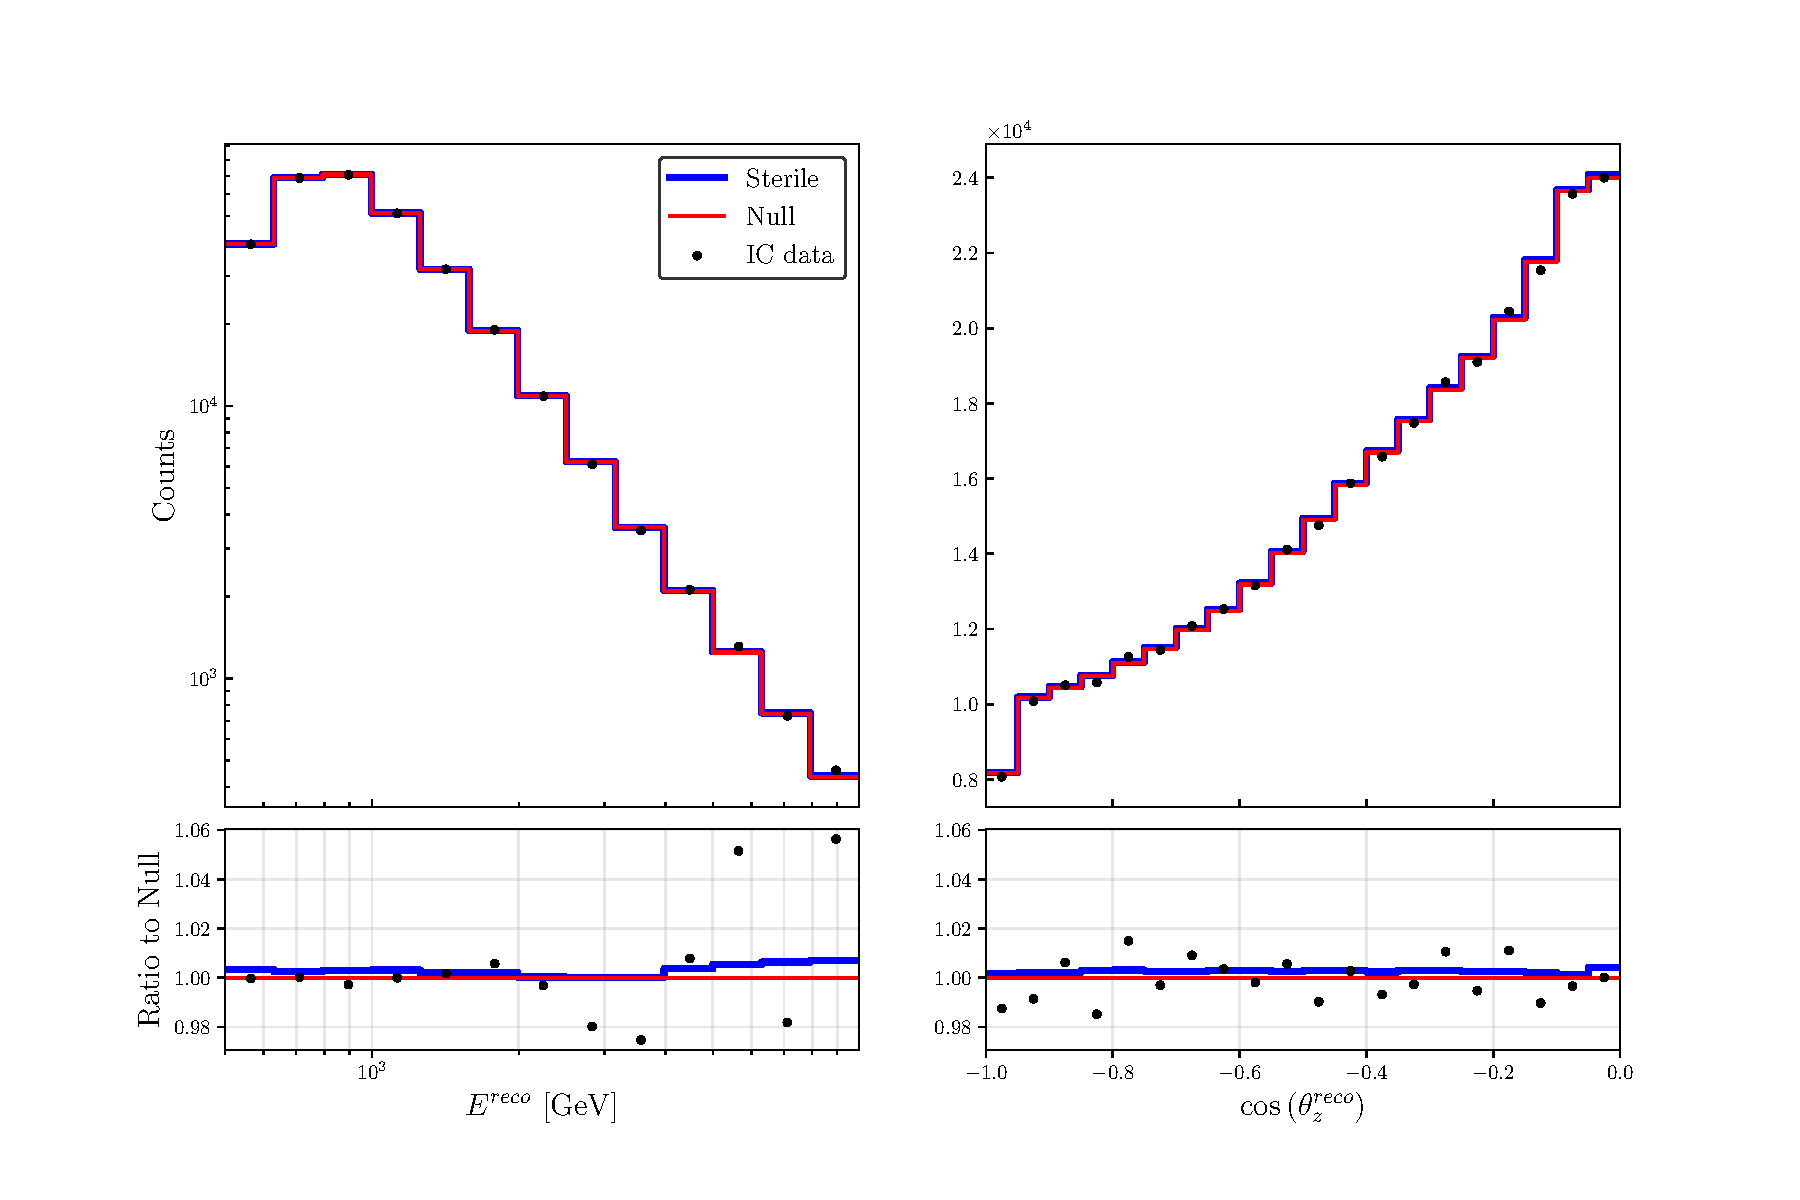
\includegraphics[width=0.8\textwidth]{figures/final_rate_plot.pdf}
    \caption{}\label{fig:final_rate_plot}%TODO: update
\end{figure}

\begin{figure}
    \centering
    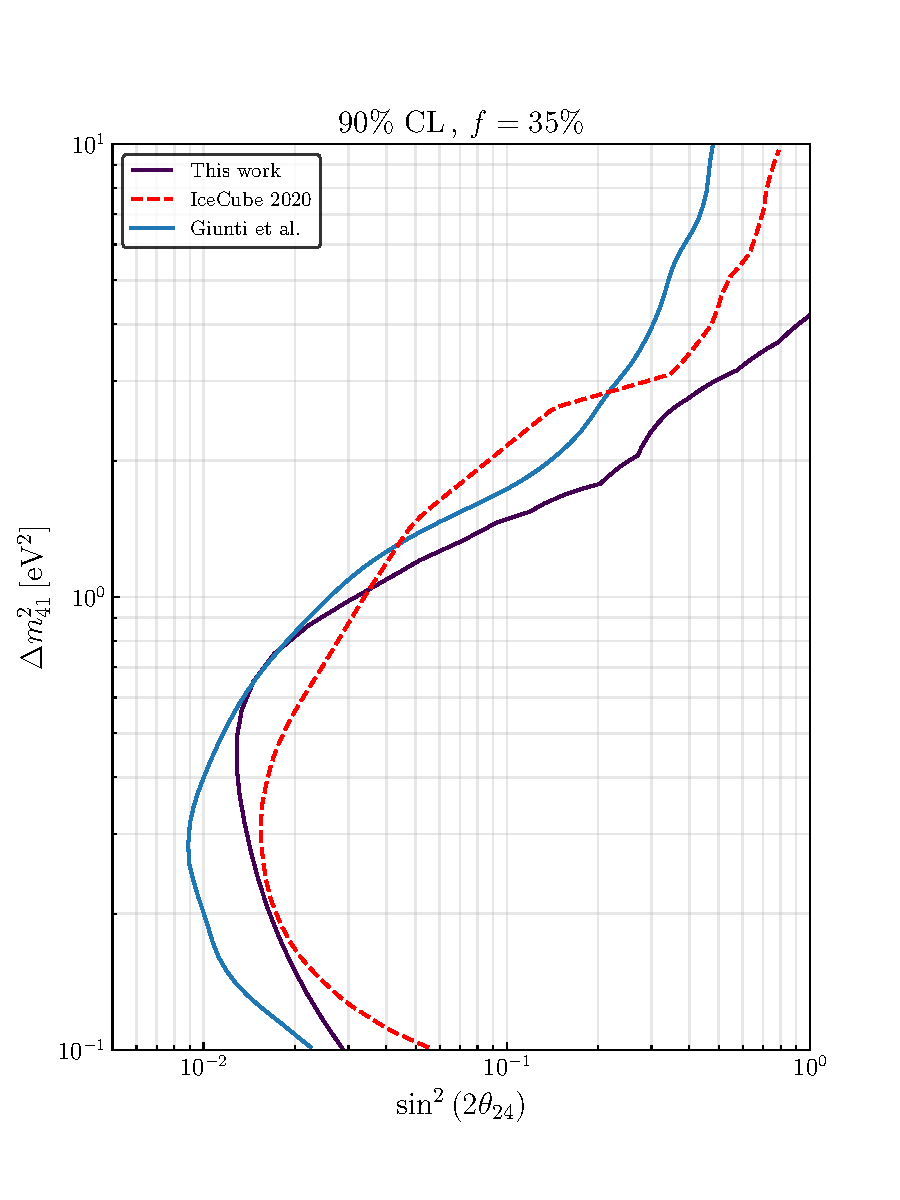
\includegraphics[width=0.8\textwidth]{figures/s24_contour.pdf}
    \caption{}\label{fig:s24_contour}%TODO: update
\end{figure}
%\end{document}